\lab{Timber Harvesting}{Timber Harvesting}
\label{lab:tv_images}
\objective{We introduce numerically solving optimal control problems with a Hamiltonian that is linear in the control through a simple tree harvesting simulation.}
\labdependencies{NumericalIVP,HIVTreatment}

\section*{Introduction}
Timber harvesting is a much needed part of business logistics management. 
Timber is the beginning of the supply chain because it provides the raw material for many housing, construction, and paper products. 
Now imagine you are the owner of a timber farm which, due to environmental regulations, can only harvest at most a fixed percentage of its trees, which must then be replanted. 
We will assume the farm operates at this fixed production rate, and we will let $x(t)$ be the amount of raw timber produced at time $t$. 

We will make the following assumptions:
\begin{itemize}
\item Growth and death rates of individual trees need not be considered
\item Tree age can be ignored (we assume harvest percentage level is low enough)
\item Amount of timber is based solely on the size of the farm (i.e. number of trees)
\end{itemize}

\subsection*{Setting Up the Problem}
In this problem, we will also assume that once the timber has been processed, it is immediately sold. 
The money can either be kept as profit or reinvested in the farm by purchasing land and labor for further tree growth. 
You, the owner of the farm, wish to find the reinvestment schedule that will maximize profit over a fixed time interval. 
We will let $u(t)$ be the percentage of timber revenue reinvested at any given time, which is our control. 
Since reinvestment in harvesting leads to more tree growth which in turn leads to more timber production, we have $x'(t) = kx(t)u(t)$, where $k$ is the return constant, which takes into account the average cost of labor and land. 
If $p$ is the market price of a unit of timber, then the profit at time $t$ is $px(t)(1-u(t))$, and the total profit is
\[p \int_0^T x(t)[1-u(t)] \, dt\]

However, we also want to take into account money which could be gained through interest on profit. This means that profit earned in year one could be placed into an interest bearing account, while profit from the end of the time period could not. In other words, money from earlier in the time period is, in some sense, more valuable. In economics, this is referred to as present-value. Now we will let $r$ be the interest rate over the period, which we will assume is fixed, so our profit, adjusted for interest, is
\[pe^{rT} \int_0^T e^{-rt} x(t)[1-u(t)] \, dt\]

The exponential term in the integral is called a \textit{discount term}. 
Notice that the function $e^{-rt}$ is a decreasing function of time, which encourages money to be invested at the beginning of the interval and future profit is discounted at a rate $r$. 
Note also that the constant $pe^{rT}$ does not affect how the integral is maximized, so we will discard it from the integral.
Therefore, our optimal control problem becomes
\begin{align}
\max_{u} \int_0^T e^{-rt} x(t)[1-u(t)] \, dt
\end{align}
subject to the constraints
\begin{align}
x'(t) &= kx(t)u(t) \\
 x(0) &= x_{0} > 0 \\
0 \leq&\; u(t) \leq 1
\label{eq:timberharvest:x}
\end{align}
In order to get a minimization problem, we negate our cost functional; the original maximization problem is equivalent to 
\[
\min_{u} \int_0^T -e^{-rt} x(t)[1-u(t)] \, dt
\]
with the same constraints.
We can then solve for the Hamiltonian, which is given by
\begin{align*}
H = \alpha f - L = kxu\alpha+e^{-rt}x(1-u)
\end{align*}
where \(\alpha\) is the costate (we have already used the usual symbol \(p\) for something else).
We can now use Pontryagin's maximum principle to obtain the costate evolution equation and the optimal control:
\begin{align}
\label{eq:timber:costate}
\alpha ' = -\frac{DH}{Dx}=u(&e^{-rt} - k\alpha) - e^{-rt}, \quad \alpha(T)=0
\end{align}
\begin{align}
\label{eq:timber:phi}
\phi = \frac{D H}{D u} &= x(k\alpha - e^{-rt})
\end{align}
If \(\phi\neq 0\), then by Pontryagin's maximum principle \(u\) is determined as the value that maximizes \(H\):
\begin{align}
\label{eq:timber:get_u_from_phi}
\text{If }\phi(t)\neq 0,\quad u(t)=\begin{cases} 1& \phi(t)>0 \\ 0 & \phi(t) < 0\end{cases}
\end{align}
On the other hand, if \(\phi=0\) on some interval, the control is singular and this does not apply.
We now wish to determine whether this can occur. 

As $x(0) = x_{0} > 0$, $k > 0$, and $u \geq 0$ for all $t$, it follows that $x'(t) = kxu \geq 0$ and $x(t) > 0$ for all $t$. 
Suppose $\phi = 0$ over some interval. 
As $x$ is strictly positive, this can occur if and only if $\alpha(t) = \frac{1}{k}e^{-rt}$ over some interval. Then, $\alpha '(t) = -\frac{r}{k}e^{-rt}$. 
However, we have that $\alpha '(t) = -e^{-rt}$ from equation \eqref{eq:timber:costate}. 
If $k \neq r$, this is clearly a contradiction. 
On the other hand, if $k = r$, then $\alpha(t) = \frac{1}{k}e^{-rt}$ for the remainder of the time interval, which contradicts $\alpha(T) = 0$. %I'm not sure this part quite holds
Thus, $\phi = 0$ cannot be sustained over an interval, and the optimal control is indeed bang-bang.

\subsection*{Solving the Problem Numerically}
Our optimal control problem is a boundary value problem.
However, the right-hand side of the ODE has discontinuities; because of this, \li{scipy.integrate.solve_bvp} has difficulty in solving it.
Since each variable has only one boundary condition, we will instead solve the problem iteratively.

In each iteration we solve the state equation forward using our current guess for the costate, and then solve the costate equation backward using our current guess for the state.
We can then update our control using our better estimates of the state and costate. 
To solve each of the differential equations, we will use the 4th-order Runge-Kutta method.
As a reminder, the RK4 method solves for the next step for the equation \(y'=f(t,y)\) as follows:

\begin{lstlisting}
def initialize_all(y0, t0, t, n):
    """ An initialization routine for the different ODE solving
    methods in the lab. This initializes Y, T, and h. """
    if isinstance(y0, np.ndarray):
        Y = np.empty((n, y0.size)).squeeze()
    else:
        Y = np.empty(n)
    
    Y[0] = y0
    T = np.linspace(t0, t, n)
    h = float(t - t0) / (n - 1)
    return Y, T, h

def RK4(f, y0, t0, t, n):
    """ Use the RK4 method to compute an approximate solution
    to the ODE y' = f(t, y) at n equispaced parameter values from t0 to t
    with initial conditions y(t0) = y0.
    
    y0 is assumed to be either a constant or a one-dimensional numpy array.
    t and t0 are assumed to be constants.
    f is assumed to accept three arguments.
    The first is a constant giving the value of t.
    The second is a one-dimensional numpy array of the same size as y.
    The third is an index to the other arrays.
    
    This function returns an array Y of shape (n,) if
    y is a constant or an array of size 1.
    It returns an array of shape (n, y.size) otherwise.
    In either case, Y[i] is the approximate value of y at
    the i'th value of np.linspace(t0, t, n).
    """
    Y,T,h = initialize_all(y0,t0,t,n)
    for i in range(n-1):
        K1 = f(T[i],Y[i],i)
        K2 = f(T[i]+h/2.,Y[i]+h/2.*K1,i)
        K3 = f(T[i]+h/2.,Y[i]+h/2.*K2,i)
        K4 = f(T[i+1],Y[i]+h*K3,i)
        Y[i+1] = Y[i] + h/6.*(K1+2*K2 +2*K3+K4)
    return Y
            
\end{lstlisting}


Lastly, we check to see if the state, costate, and control have converged.
We will check if the relative change for each of the state, costate, and control is less than \(\delta = 0.001\).
Use the following code to start:

\begin{lstlisting}
import numpy as np
from matplotlib import pyplot as plt

def solve_tree_harvest(x0, k, r, T, N=1000, delta=0.001):
    """
    Solves for the optimal control for the tree harvesting problem 
    with the given parameters.
    
    Parameters:
    """
    t = np.linspace(0,T,N+1)
    h = T/N
    h2 = h/2
    
    x = np.zeros(N+1)
    alpha = np.zeros(N+1)
    u = np.zeros(N+1)
    
    while True:
        ## Solve for x, alpha, and u
        # put code here
        
        # Check for convergence
        if (np.sum(np.abs(oldu - u)) < delta*np.sum(np.abs(u))
           and np.sum(np.abs(oldx - x)) < delta*np.sum(np.abs(x))
           and np.sum(np.abs(oldalpha - alpha)) < delta*np.sum(np.abs(alpha))):
            break
            
\end{lstlisting}

\begin{problem}
Write a function that takes as input scalars $x_{0}$, $k$, $r$, and a final time $T$ and solves the optimal control problem stated above using the RK4 method described above. The function will return the time-step and the values of x and u at the specific time-steps. 

Hint: Solve for $x$ using the RK4 code and equation \eqref{eq:timberharvest:x}. Solve for $\alpha$ using the RK4 code and and equation \eqref{eq:timber:costate}. Use equation \eqref{eq:timber:phi} to solve for $\phi$. Finally, use equation \eqref{eq:timber:get_u_from_phi} to get a new solution vector of $u$'s.

Another hint: You may need to reduce the step size in updating $u$ in order for the iterative method to converge. If so, use 
\[u_{real\text{ }new} = (u_{new} + u_{old}) / 2.\]

Yet another hint: Remember that $\alpha$ is solved for backwards, so remember to switch it.

\end{problem}

\begin{problem}
\label{prob:timber:solve_ode1}
Using your function from problem 1, plot time vs timber production ($x$) and plot time vs reinvestment percentage ($u$) for the following values: $x_{0} = 100$, $k = 1$, $r = 0$, and $T = 5$.

\end{problem}
\begin{figure}[H]
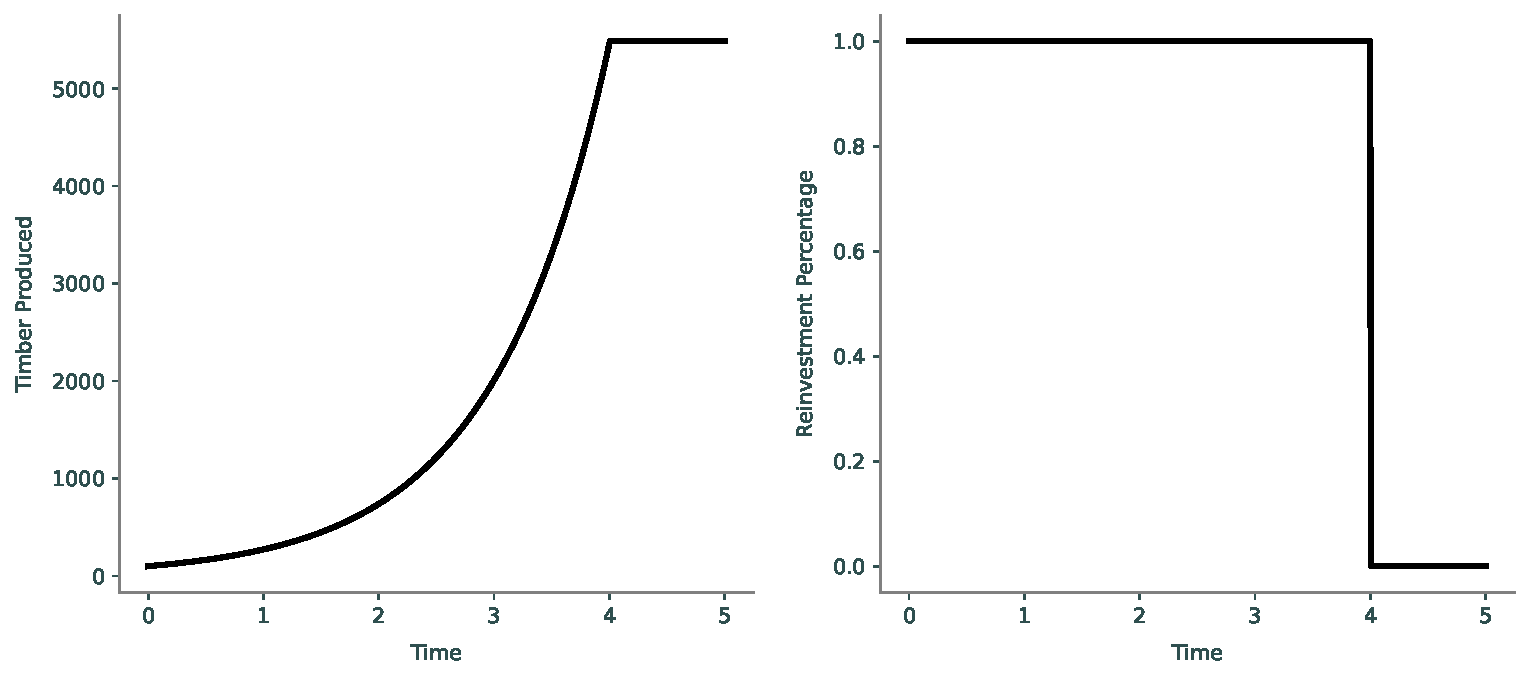
\includegraphics[width=\textwidth]{figures/Example_problem2.pdf}
\caption{The solution for problem \ref{prob:timber:solve_ode1}.}
\end{figure}

In the graph you just plotted, you will notice that in the control the graph is continuous and there is an abrupt shift at $t = 4$. 
We knew this problem was bang-bang, and the vertical section of the graph at $t = 4$ represents the switching point. 
We can also notice that $x(t)$ is exponential for $0 \leq t \leq 4$ and constant for $4 \leq t \leq 5$, as we would expect. 
Thus, in this scenario the optimal reinvestment strategy is to reinvest all timber revenue for the first four-fifths of the time interval, allowing the farm to grow. Towards the end of the time interval, all revenue should instead be kept as profit.

\begin{problem}
\label{prob:timber:solve_ode2}
Plot the same graphs that you did in problem 2, but instead for the following values: $x_0 = 100$, $k = 0.3$, $r = 0.05$, and $T = 5$. At what time does the switching point occur?

\end{problem}
\begin{figure}[H]
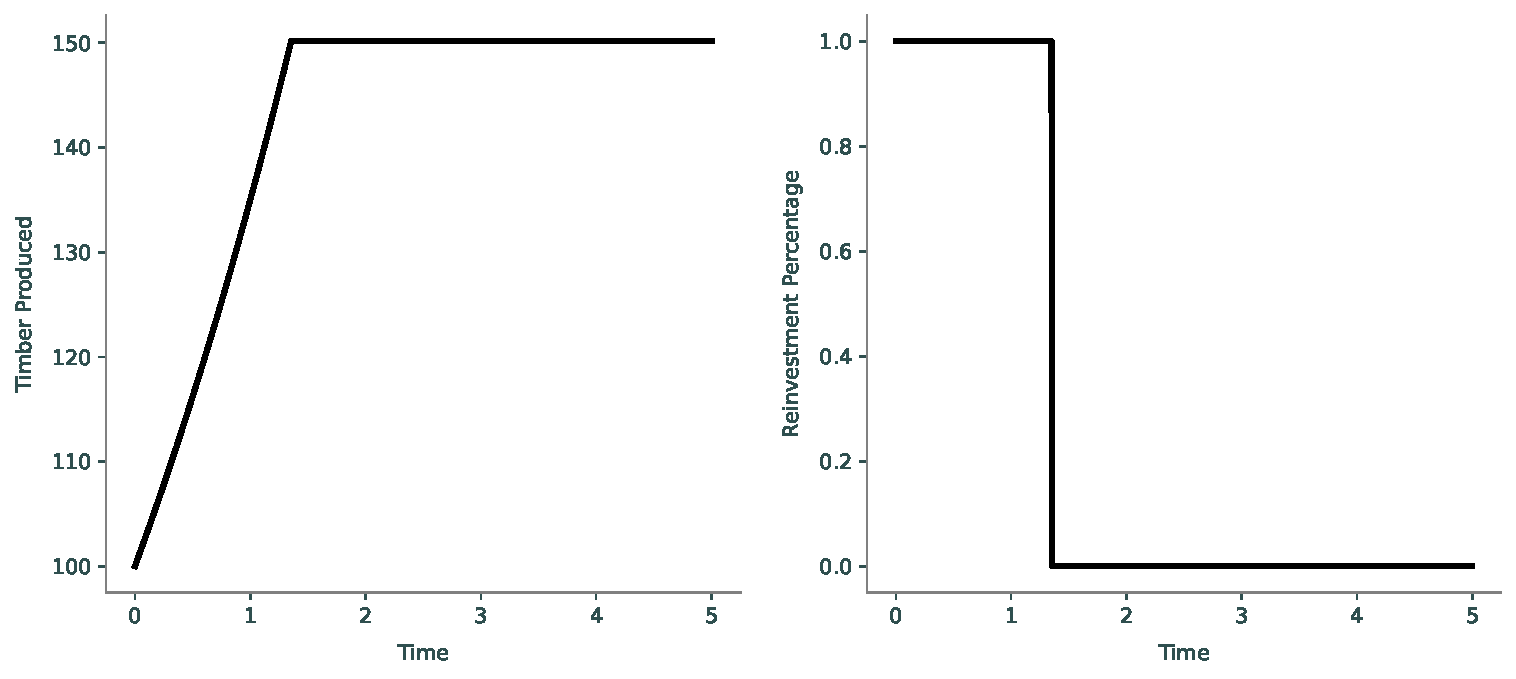
\includegraphics[width=\textwidth]{figures/Example_problem3.pdf}
\caption{The solution for problem \ref{prob:timber:solve_ode2}.}
\end{figure}


\begin{problem}
Now use the same parameters as in problem 3, but vary the initial value of the timber production capacity ($x_{0}$). 
You should try a smaller value, a slightly larger value, and fairly larger value for $x_{0}$.
What do you notice about the optimal controls? 
Are they the same or are they different?

\end{problem}


